\section{Introduction}
\label{sec:introduction}

Modern industrial ecosystems rely on complex, multistage transformations that convert naturally occurring raw materials into intermediate chemicals and ultimately into advanced technological products. Understanding the pathways connecting raw material extraction to refined intermediates and high-value products is crucial for identifying vulnerable dependencies in global supply chains, assessing critical mineral risks, and discovering alternative production routes during disruptions.

Traditional supply chain analysis predominantly employs top-down approaches that trace backward from finished products through supplier networks. However, these methods face significant limitations due to opaque supplier networks and proprietary manufacturing processes that obscure intermediate dependencies~\cite{colon2022systemic}. Recent real-world disruptions have demonstrated the critical consequences of these analytical blind spots~\cite{hasan2022demand, chakraborty2022empirical, tam2022understanding}.

Such dependencies can be studied more systematically through knowledge graph (KG) representations.
KGs have been constructed in various domains, including medicine~\cite{brbic2024predicting}, biology, and material sciences~\cite{venugopal2024matkg, mrdjenovich2020propnet}.
For instance, knowledge graphs in material sciences~\cite{venugopal2024matkg}, extract relationships between 
the complete space of materials and their properties and applications, processes and methods for synthesis, and other characteristics.
These provide a systematic approach to organizing scientific data and allow researchers to analyze and understand material science datasets, and discover new types of processes and materials.
Until recently, such knowledge graphs were extracted automatically using standard natural language processing methods, from well-structured scientific publications~\cite{Stocker2023Creating, Dessi2021Generating}.

However, KG construction is more difficult in the case of supply chain networks for multiple reasons. 
First, material classes are less structured, as they include inputs for diverse contexts, such as industry, not just laboratories.
Second, data is available in a broad range of documents, including public literature, patents, and technical references, in addition to scientific publications.
Therefore, a new class of KGs are needed to provide a foundation for evidence-based network construction that avoids the opacity constraints of top-down approaches.
Finally, graph representations are insufficient for many of these processes, as they involve transforming a set of inputs into a set of outputs, and non-binary relations must be considered.
A hypergraph representation is more suitable for such information, and has been proposed in the literature \cite{wolf2016advantages, fatemi2019knowledge, luo2025hypergraphrag}.
Wolf et al.~\cite{wolf2016advantages} show that ``hypergraphs better model complex, non-pairwise relationships, are computationally more efficient, and can represent temporal and locality effects, unlike binary graphs''. Luo et al.~\cite{luo2025hypergraphrag} demonstrate that hypergraph knowledge representation provides ``knowledge completeness, structural expressiveness, and inferential capability'' superior to binary graph approaches.
Fatemi et al.~\cite{fatemi2019knowledge} show that knowledge hypergraphs are a solution to the problem that traditional binary knowledge graphs cannot adequately represent relations involving more than two entities, even though over one-third of entities in real-world knowledge bases participate in such non-binary relations. While some previous research has been conducted separately applying knowledge graph theory~\cite{kosasih2022towards, almahri2024enhancing} and hypergraph approaches to the mapping of supply-chains~\cite{suo2018exploring, li2023research}, an approach utilizing knowledge hypergraphs (KHGs) has not yet been developed.

%Knowledge hypergraphs have not been developed for supply chain networks, especially using diverse kinds of unstructured datasets which contain such information. 
%\anil{some more discussion, citations}

% In contrast, a bottom-up approach begins with naturally occurring materials and systematically follows documented industrial transformations to construct complete transformation networks. This methodology leverages the fact that upstream industrial processes are often well-documented in public literature, patents, and technical references, providing a foundation for evidence-based network construction that avoids the opacity constraints of top-down approaches.



% This paper presents a bottom-up agentic AI approach for constructing 
% % \textbf{Material Evolution Graphs} (MEGs). 
% \emph{Material Evolution Knowledge Hypergraph} (\tool{}).
% A Material Evolution Graph (MEG) \mlwcomment{This looks weird, defining two different terms as "MEG" (especially since one of them does not abbreviate to MEG). We should be consistent in our terminology and only use MEG for one term (and ideally only define it once -- yesterday "MEG" was defined multiple times.)} maps material transformation pathways from naturally occurring forms (ores, mineral compounds, and brines) through 
% processing stages to their eventual form for use in technological products. The MEG serves as the foundational component for constructing a full \sout{\textbf{Technology Dependency Network} (TDN)} supply chain network that systematically maps industrial transformation pathways from naturally occurring raw materials through to their eventual use in the manufacture of advanced technological products. \samarth{Maybe we should avoid discussion of TDNs here, since we don't have a published paper we can point to.}. \adscomment{It used to all say TDN. Was trying to massage it. I agree, probably don't want TDN, but will need to say what it is used for.} \sout{A TDN is a multi-level, hierarchical representation that systematically delineates the interdependencies underpinning the development and maintenance of a specific technology. Formally, we define a TDN as a directed acyclic multipartite relational graph $G(V, E)$ with known levels $L_1, L_2, \ldots, L_k$, where each level represents a separate dependency tier ranging from complete technologies to components, materials, and producing countries. Vertices are formed as a union of subsets of $L_1, \ldots, L_k$, with edges connecting lower levels to higher levels: $\bigcup_{i=1}^{k-1} L_i \times L_{i+1}$. Each edge has weight $w_{uv} > 0$ indicating the influence input $u$ has on production of $v$. For country-to-material edges, weights represent production proportions.}

\noindent
\textbf{Our Contributions.}\\
(1) We present a bottom-up agentic AI approach for constructing a 
\emph{Material Evolution Knowledge Hypergraph} (\tool{}), a labeled directed multi hypergraph for representing how material transformation processes transform a set of inputs to outputs through 
processing stages to their eventual form for use in technological products.
Such information cannot be represented through standard knowledge graphs~\cite{venugopal2024matkg, mrdjenovich2020propnet}.
\tool{} serves as the foundational component for constructing a full  supply chain network that systematically maps industrial transformation pathways from naturally occurring raw materials through to their eventual use in the manufacture of advanced technological products. We refer to the process of building an MEKH as the \processname{} (\process{}).

\iffalse
\begin{figure}[h]
    \centering
    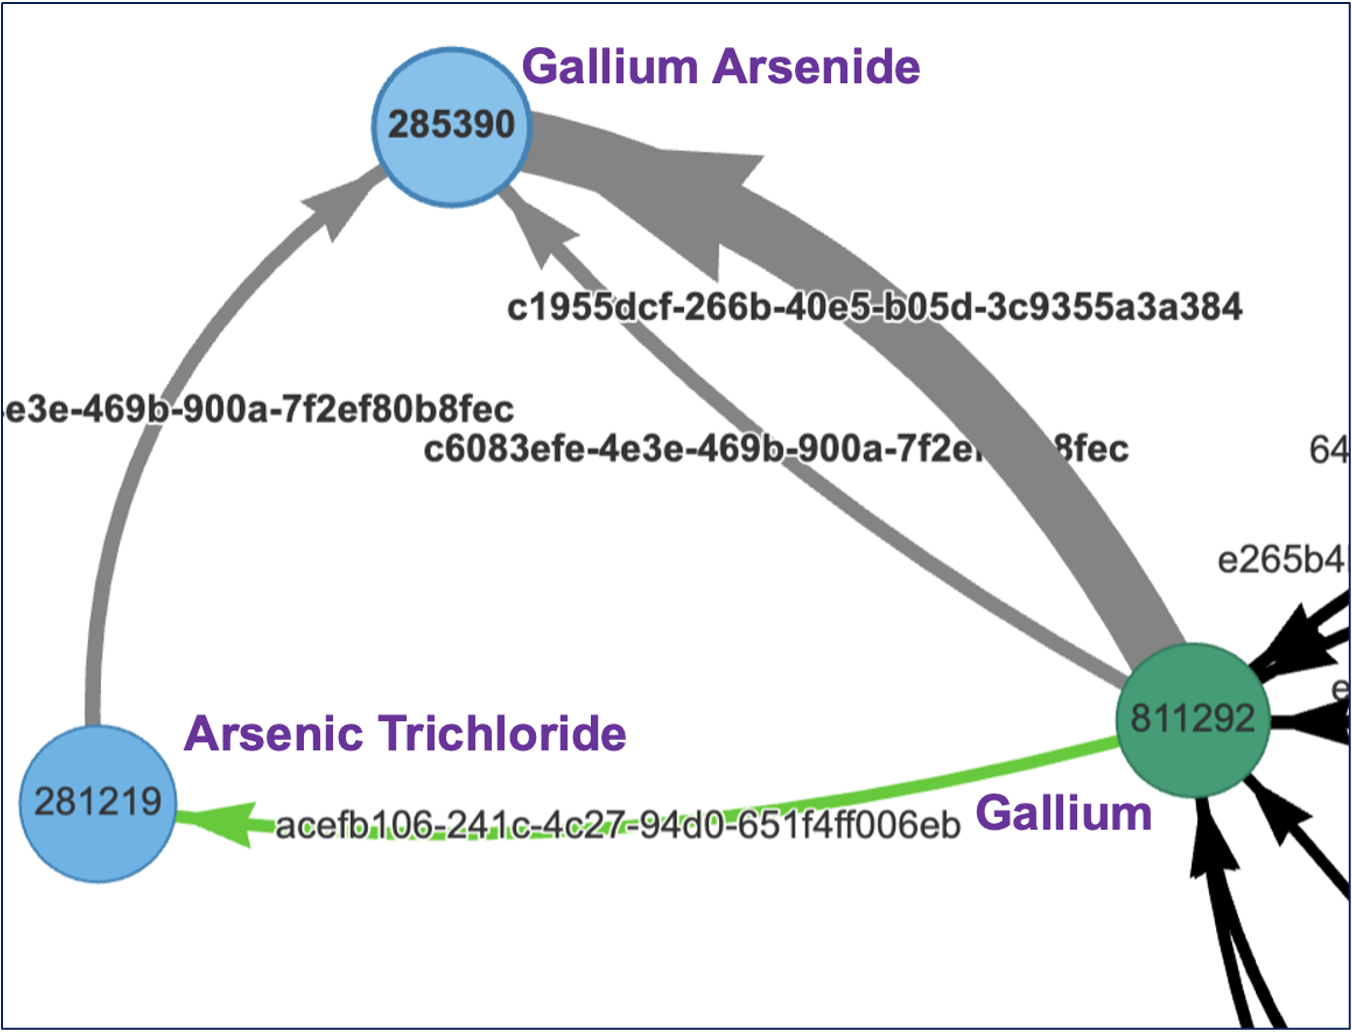
\includegraphics[width=0.9\linewidth]{images/gallium-arsenide.png}
    \caption{Partial \tool{} showing example relationships between a mineral and multiple compounds, each with a different assigned HS Shipping Code. \samarth{We need some more detail. Perhaps a visualization of the whole network, with this bit shown in an inset?} \samarth{actually, given Fig.~\ref{fig:pipeline}, do we need this one?}
    \adscomment{I was just trying to provide a visual to break-up a long text section. With Fig 4, probably don't need.} \mlwcomment{If we do keep, probably need a legend}}
    \label{fig:pipeline}
\end{figure}
\fi


\iffalse
We employ a multi-agent architecture in which specialized LLM agents discover, classify, and validate materials and industrial processes. 
By representing supply chains as directed hypergraphs that accommodate multi-input, multi-output industrial processes, the system constructs traceable, evidence-backed networks that reveal transformation pathways from naturally occurring materials to advanced technological products.
\anil{some overlap with earlier para}
\fi


\process{} involves an iterative, bottom-up discovery.
The pipeline begins with raw inputs and expands through multiple 
iterations to cover entire transformation chains, uncovering intermediates that are invisible in top-down analyses.
We develop tools for LLM-assisted reasoning for scalable knowledge extraction, where specialized agents discover, classify, and validate materials and processes from unstructured references. 
Each transformation edge is supported by multiple references, scored for source quality and content relevance, enabling trustworthy networks, providing 
evidence-backed process validation.

\noindent
(2) We use our approach to construct \tool{}s for some of the critical minerals used in microelectronics, for example, Boron.
\tool{} identifies all key routes from ore to advanced compounds.
We analyze structural properties of these hypergraphs, and notions of criticality of materials involved. 
This can guide supply chain resilience planning, and can reveal alternative routes for strategic materials.

% \noindent
% \textbf{Contributions:} 
% \samarth{need to expand and itemize; we have multiple contributions}
% \sout{The key contribution of this work lies in demonstrating how agentic AI systems can overcome the fundamental limitations of traditional supply chain analysis by systematically constructing bottom-up material transformation networks. Unlike top-down approaches that encounter opacity barriers, or manually curated knowledge graphs that lack scalability, this automated approach scales to complex industrial networks while maintaining traceability to verifiable sources. The resulting networks enable critical mineral pathway analysis, bottleneck identification, and supply chain resilience planning by revealing alternative production routes and intermediate dependencies that remain hidden in conventional analyses.}

% This pipeline contributes several key innovations:

% \begin{enumerate}
%     \item We formalize supply chain transformations as a directed hypergraph. This naturally represents 
%     realistic processes with multi-input, multi-output structures, unlike simple graph models.
%     \item Iterative, bottom-up discovery: the pipeline begins with raw inputs and expands through multiple 
%     iterations to cover entire transformation chains, uncovering intermediates that are invisible in top-down 
%     analyses.
%     \item LLM-assisted reasoning for scalable knowledge extraction: Specialized agents discover, classify, and validate materials and processes from unstructured references.
%     \item Evidence-backed process validation: Each transformation edge is supported by multiple references, scored for source quality and content relevance, enabling trustworthy networks.
% \end{enumerate}

% This work enables:

% \begin{itemize}
%     \item Critical mineral pathway analysis—understanding all possible routes from ore to advanced compounds.
%     \item Identification of bottlenecks—finding intermediate compounds that connect multiple downstream technologies.
%     \item Supply chain resilience planning—revealing alternative routes for strategic materials.
% \end{itemize}